\chapter{Taxonomy}\label{sec-taxonomy}
In this chapter, we first introduce two existing taxonomies given by Segel and Heer ~\cite{Segel2010} and Tong et al. ~\cite{Tong2018}, respectively. The former is a highly cited paper and has contributed greatly to narrative visualization, while the latter is an up-to-date survey on storytelling and visualization adding a variety of new narrative methods and works. We aim to demonstrate their primary characteristics for an overview instead of explaining the technical details of each taxonomy. After that, we propose our taxonomy derived from the definition of the term "narrative". 

\section{Taxonomy by Segel and Heer}

Segel and Heer \cite{Segel2010} investigated 58 examples of narrative visualizations and formulated a design space containing three divisions of features, namely, genres, visual narrative tactics, and narrative structure tactics. 

\begin{figure}[H]
	\centering 
	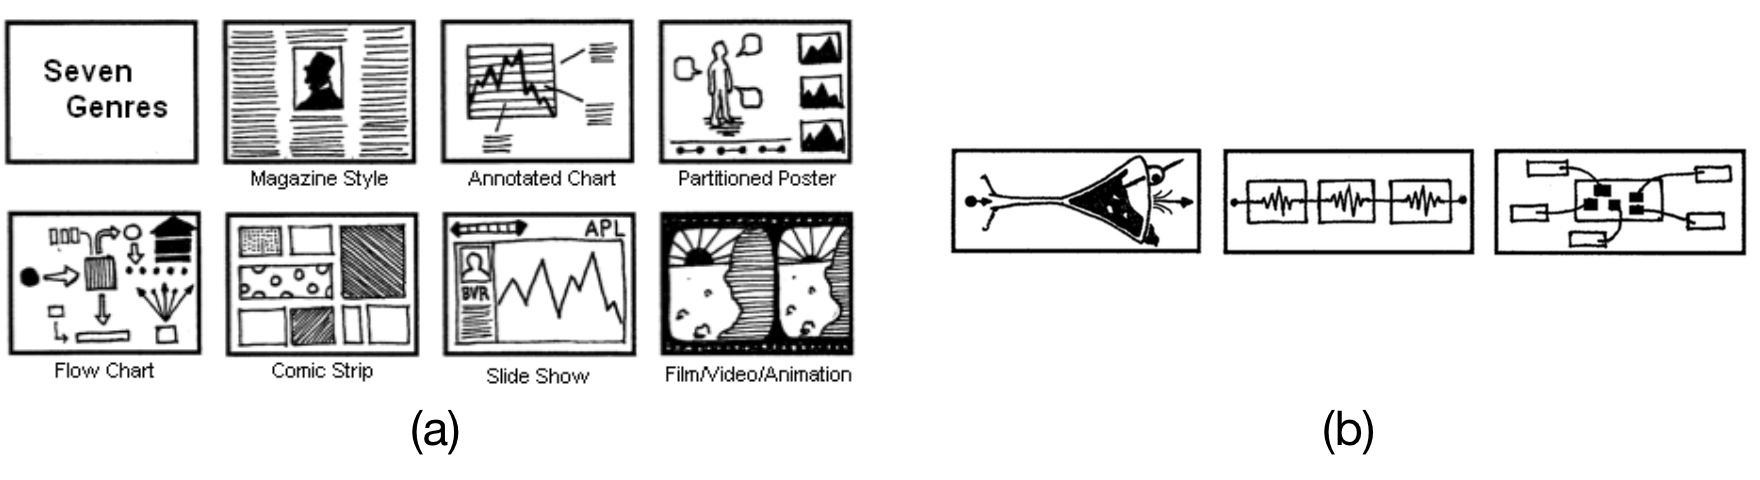
\includegraphics[width=0.9\textwidth]{figure/taxonomy1.png} 
	\caption{(a) Seven genres of narrative visualization. (b) Three schemes of structure. Left: martini glass style; middle: interactive slideshow; right: drill-down story \cite{Segel2010}. } 
	\label{taxonomy1} 
\end{figure}

\begin{compactitem}
	\item \textbf{Genres.} The first division identifies seven basic genres shown in Figure \ref{taxonomy1}(a): magazine style, annotated chart, partitioned poster, flow chart, comic strip, slide show, and film/video/animation.   These genres differ in the number of frames and the ordering of visual elements. 
	
	\item \textbf{Visual Narrative Tactics.} The second division concerns visual mechanisms to facilitate the narrative. These methods are subdivided into three sections. \textit{Visual structuring} describes the way to organize the story and points out the current position of the viewer through visualization (e.g., progress bars). \textit{Highlighting} directs attentions to the emphasized elements using color, motion, etc. \textit{Transition guidance} aims to avoid disorienting the viewer when changing scenes.
	
	\item \textbf{Narrative Structure Tactics.} The third division considers both visual and non-visual techniques to assist the narrative. These ideas are captured in a three-way classification. \textit{Ordering} corresponds to sequences viewers look at through narratives, including linear path, random access, and user-directed path. \textit{Interactivity} allows viewers to manipulate the visualization, while \textit{messaging} displays how visualization communicates insights with viewers combined visual cues and text descriptions (e.g., annotations). 
	
\end{compactitem}

This paper further characterize these design differences in term of the balance between author-driven and reader-driven approaches together with messaging and interactivity. Three common schemes can be classified as shown in Figure \ref{taxonomy1}(b). \textit{Martini glass structure} begins with an author-driven introduction to the narrative, followed by a reader-driven stage to allow interactive exploration. \textit{Interactive slideshow} incorporates interactions within each slide, promoting a dialogue between these two approaches. \textit{Drill-down story} allows readers to choose instances from a given theme, which prioritizes the reader-driven approach.

Though Segel and Heer offered a nice framework and first identified seven genres of narrative visualization, this work is more than 8 years old. The past few years have witnessed some newly emerging formats (e.g., ScrollyTelling \cite{scrollytelling} and SketchStory \cite{Lee2013}) and a gradual shift of existing genres. These changes require a study on recent advancements in narrative visualization. 

\section{Taxonomy by Tong et al.}

Tong et al. \cite{Tong2018} conducted a survey targeting at storytelling literature in visualization, which is much more up to date and shows the evolving field. Besides, instead of a focus on journalism like Segel and Heer \cite{Segel2010}, the authors provided a comprehensive survey of storytelling literature with a coverage of scientific visualization, information visualization, and geo-spatial visualization. 

In this survey, storytelling is considered both as an entity and a creative process. Thus, the taxonomy is first based on the logical notations of who, how, and why. 

\begin{compactitem}
	\item \textbf{Who} plays the main role in storytelling for visualization? This survey identifies two dimensions, namely, \textit{authoring tools} and \textit{user engagement}. The former addresses the author who crafts the story, while the second is about the audience. 
	
	\item  \textbf{How} are stories told? Two categories are classified, i.e., \textit{narrative} and \textit{transition}. Transitions can be further subdivided into animated and static transitions. 
	
	\item \textbf{Why} use storytelling for visualization? \textit{Memorability} and data \textit{interpretation} are important goals for storytelling. They address why authors present data in the form of stories.

\end{compactitem}

The second dimension of this taxonomy refers to the sequence of events, which tracks the viewing path of readers through a narrative. Four categories are extracted. \textit{Linear} indicates that viewers are supposed to follow the order prescribed by the author, while \textit{user-directed path} allows readers to select or create the path. \textit{Parallel} visualizes multiple paths at the same time, and \textit{random access} (also known as \textit{overview}) means no prescribed path. 

The taxonomy in Figure \ref{taxonomy2} presents an overview of important elements in storytelling visualization. However, several dimensions still seem vague and intertwined. For example, as the paper stated itself, "narrative visuals contain the transitions between events", it is hard to distinguish \textit{transition} from \textit{narrative} when categorizing literacy in \textit{how}. In addition, there is no work belonging to \textit{interpretation} in this survey. 

\begin{figure}[H]
	\centering 
	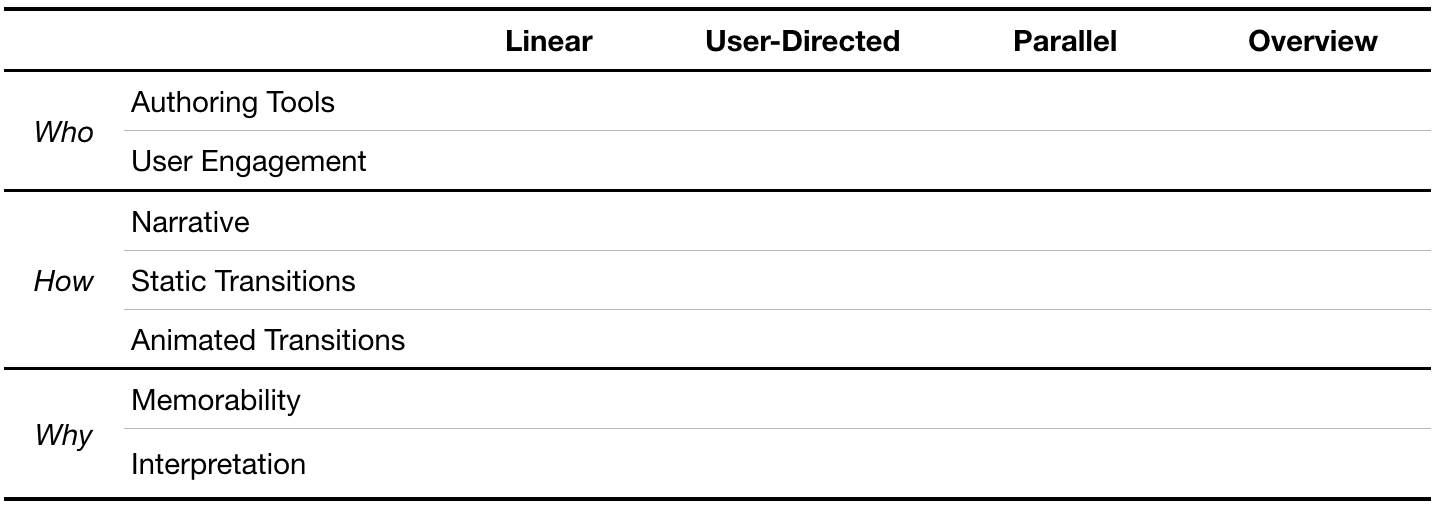
\includegraphics[width=0.95\textwidth]{figure/taxonomy2.png} 
	\caption{ The classification of the storytelling literature proposed by Tong et al. \cite{Tong2018} } 
	\label{taxonomy2} 
\end{figure}

\section{Taxonomy for Visual Design in Data-driven Storytelling}

Segel and Heer \cite{Segel2010} took an empirical approach to investigate the design from an analysis of visualizations. Several works \cite{Bach2018, Stolper2016, McKenna2017} have furthered this line of research and enriched the design space with emerging narrative techniques. However, the capability of visualization practitioners like data journalists to produce artifacts is limited to authoring tools, which did not cover cutting-edge techniques to make compelling stories. Tong et al. ‘s taxonomy did not specify concrete techniques to compose a story. 
%In recent years, we have seen the design space of narrative visualization studied by several academic works as in the above surveys. Most of them \cite{Bach2018, Stolper2016, Segel2010} provided design choices by analyzing existing stories found on popular websites. Since there is a lack of evaluation for the effectiveness of these stories, extracted techniques and their roles in storytelling might not be so faithful and comprehensive.  
Therefore, in this taxonomy, we consider the fundamental components of stories and explore designs with a look into visualization practices and researches. Firstly, in view of the term "narrative", the definition in the Oxford English Dictionary \cite{oed} is "an account of a series of events, facts, etc., given in order and with the establishment of connections between them". Following this explanation, we propose our taxonomy for visual design in data-driven narratives, which consists of three components.


\begin{compactitem}
	\item \textbf{Scene}. The "scene" component concerns the explanation of data and the communication of messages. \textit{Visualization types} work closely in conjunction with data. Despite diverse custom visualizations depending on different tasks, a few types appear frequently, e.g., maps, bar charts, and pictographs. \textit{Textual annotation} includes descriptions beyond and on visualization, which assists both in narration and interpretation. \textit{Highlighting} performed by changing graphical properties or leveraging close-up techniques draws readers' attention to the emphasized elements.
	
	\item \textbf{Sequence}. The second component reflects on the author-specific ordering in storytelling, which imposes a structure to a story and enhances the navigation for readers. \textit{Linear} narratives are typical in data-driven storytelling. \textit{Non-linear} narratives are well received in movies, which shed light on the design of visual data stories. 

	\item \textbf{Transition}. The third component links separate story scenes with attractive visual effects. To convey a story smoothly, many techniques are explored such as camera motions, temporal and spatial controls, animated transtions, morphing, and metaphors. 
\end{compactitem}

Our taxonomy tries to better explore and summarize the content and representation of each story component. Thus, it could facilitate visualization selections. The organization of a story is somehow analogous with PowerPoint slides: each scene can be considered as a slide; the sequence indicates how authors organize multiple scenes or slides in a certain order; and the transitions are similar to visual effects when switching from one slide to another. Actually, some works, especially surveys, may address more than one theme. We have to recognize subjectivity when categorizing a diverse set of designs into a taxonomy and placing them by what we determine to be the main focus of the work. The detailed visual design techniques are described in Chapter 3.


\newpage